%\subsection{Ejercicio 1}\label{subsec:ej1}

En este primer ejercicio se ha creado una escena que incluye dos tipos de árboles (un árbol de copa redonda y un pino), una pelota, el suelo y un sol.

Para no tener problemas con la superposición en los árboles primero se dibuja el tronco, y a continuación las hojas. De esta forma las hojas tapan un poco al tronco, dando realismo. Para dibujar el árbol de la izquierda se han usado varios círculos rellenos, con distinta posición y distinto radio. Para ello se ha usado la función \textit{arc}. \\

Para el pino (árbol a la derecha) se han usado triángulos de distinto tamaño:
\begin{lstlisting}[language=PostScript, caption=Pino, captionpos=b, label=fun:pino]
% Hojas de abajo
newpath
    0.3 0.7 0 setrgbcolor  % Color verde
    285 90 moveto         
    230 0 rlineto
    -115 310 rlineto
    closepath
    fill
stroke

% Hojas de medio-bajo
newpath
    0.3 0.7 0 setrgbcolor  % Color verde
    300 150 moveto         
    200 0 rlineto
    -100 250 rlineto
    closepath
    fill
stroke

% Hojas del medio-alto
newpath
    0.3 0.7 0 setrgbcolor  % Color verde
    315 210 moveto         
    170 0 rlineto
    -85 190 rlineto
    closepath
    fill
stroke

% Hojas de arriba
newpath
    0.3 0.7 0 setrgbcolor  % Color verde
    330 270 moveto         
    140 0 rlineto
    -70 130 rlineto
    closepath
    fill
stroke
\end{lstlisting}
Se puede observar que para cada triángulo la coordenada $Y$ es mayor, para que esté situado un poco más arriba que el anterior.\\

También se han usado distintos colores para las hojas del árbol de copa redonda para dar sensación de luz, sombras y hojas nuevas. Se ha aplicado color a todos los elementos con \textit{setrgbcolor}, mezclando valores del `0' al `1' para los canales Rojo, Verde y Azul.\\

En la esquina superior derecha se ha dibujado un \textbf{sol con rayos}:
\begin{lstlisting}[language=PostScript, caption=Sol, captionpos=b, label=fun:sol]
newpath
    1 0.83 0 setrgbcolor  % Color amarillo-naranja
    600 750 40 0 360 arc % Pintar círculo cerca de la esquina superior derecha
stroke
\end{lstlisting}
Para dibujar el círculo del sol se usa la instrucción \textit{arc} pero no se ve entero porque se ha colocado en el límite ($x=600$). Otra opción sería cambiar el prámetro $360$ por los grados concretos de la circunferencia.\\

Para pintar los rayos de luz del sol se pintan tres rayas con un grosor \textit{5 setlinewidth} porque es el que se ha dado a la pelota y no se ha modificado posteriormente. Se sitúa el ``lápiz'' en $X = 550$ y se mueve hacia la izquierda $80$ unidades. Como se han dibujado 3 rayos, se necesitan tres bloques que cambien el valor de la componente $Y$:
\begin{lstlisting}[language=PostScript, caption=Rayos del sol, captionpos=b, label=fun:rayos_sol]
% Rayos del SOL
newpath % Rayo horizontal
    1 0.83 0 setrgbcolor  % Color amarillo-naranja
    550 750 moveto
    -80 0 rlineto
stroke

newpath % Rayo oblicuo arriba
    1 0.83 0 setrgbcolor  % Color amarillo-naranja
    550 780 moveto
    -80 25 rlineto
stroke

newpath % Rayo oblicuo abajo
    1 0.83 0 setrgbcolor  % Color amarillo-naranja
    550 720 moveto
    -80 -25 rlineto
stroke
\end{lstlisting}

A continuación se muestra la imagen obtenida\myref{fig:1ejer1}:
\begin{figure}[H]
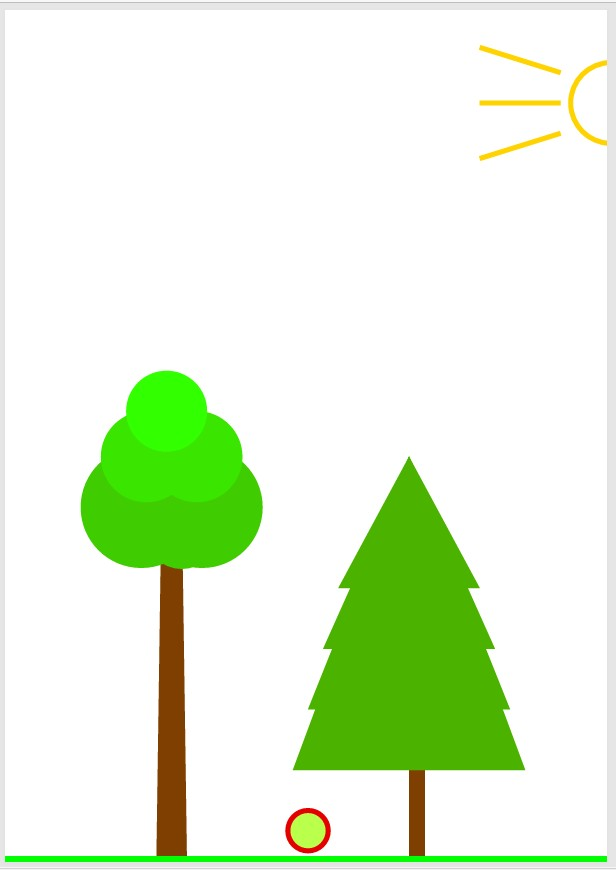
\includegraphics[width=0.8\textwidth]{images/ejer1_completo.jpg}
\caption{Propuesta ejercicio 1}
\label{fig:1ejer1}
\end{figure}

Como \textbf{ampliación} para los árboles se podrían dibujar las ramas que sujetan las hojas en el de copa redonda. O dibujar algún fruto como unas manzanas (círculos rojos). Para el pino se podría haber decorado como un pino de Navidad. Otra opción de mejora sería darle realismo a la pelota haciéndole los dibujos de una pelota de tenis o baloncesto. Por último, se podrían incluir algunas nubes o pájaros en el cielo.\\
 
El código completo se puede ver en el anexo \ref{anexo:ej1}. En el anexo \ref{anexo:pdf1} se puede ver la página pdf generada.
